\documentclass[a4paper]{IEEEtran}
\usepackage[utf8]{inputenc}
\usepackage{color}
\usepackage{graphicx}
\usepackage{mwe}
\usepackage{amsmath}
\usepackage{booktabs}
\usepackage{multicol}

\title{Malware Analysis Report\\\Large{``Sample2.exe''}}
\author{
    \begin{tabular}{lr}
        Contro Filippo &VR437055\\
        Martini Michele &VR437056
    \end{tabular}
}

\begin{document}
	\maketitle
	\section{Executive summary}
	The malware ``Sample2.exe'' shows itself as a calculator app, with the appropriate icon and the expected behavior. Once it is opened by the user there is a simple GUI to perform basic arithmetic operations. Under the hood, however, the malware deactivates the Windows security center, makes many POST request to various internet sites and infects many other files in different locations, from the local folder to the system application's executable.
	
	The whole analysis process has been done on the provided virtual machine, which runs Windows 7 as operating system and contains a bunch of tools to make both static and dynamic analysis. The reverse engineering instead has been done on local machines.
	
	\section{Static analysis}
	We began the static analysis using \emph{PEStudio}\footnote{https://www.winitor.com/}, a tool which performs malware initial assessment, studying headers, sections and many other features of the executable, which is never executed.
	This first analysis gave us many indicators of probable malicious behavior.
	First of all, in the main view we noticed an \emph{entropy} value greater than 7, therefore it's likely that either the file has been packed or some sections has been obfuscated. Entropy is a measure of the order of the application, and it is calculated with statistical operations on the bytes; As explained in this article\footnote{http://n10info.blogspot.com/2014/06/entropy-and-distinctive-signs-of-packed.html} 
	
	``When a section of code of a file is compressed, the total entropy will increase while counting, i.e. , it will get closer to the standard sum of all bits - this will mean higher efficiency of information storage, i.e., possible compression of section of code.

	\begin{figure}[htp]
		\frame{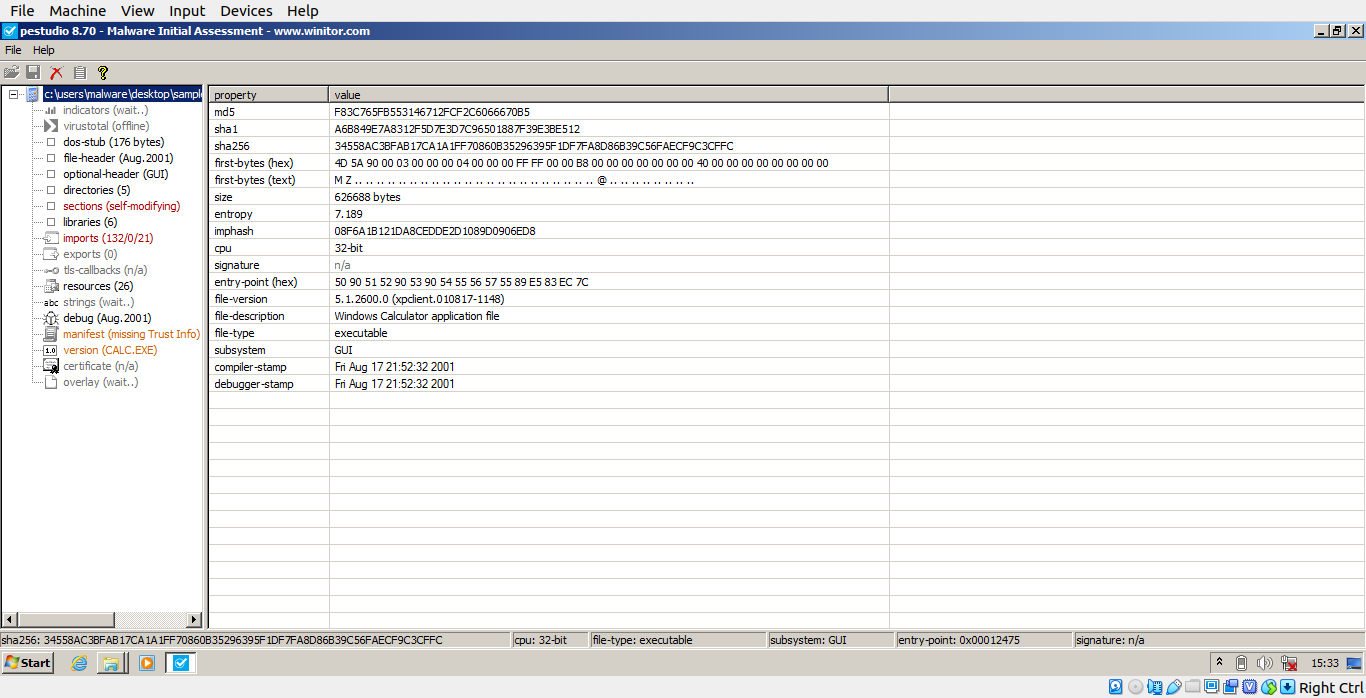
\includegraphics[width=0.5\textwidth]{img/PEStudio-main.png}}
	\end{figure}

	The maximum value for entropy in PEStudio is 8, so this high value is a clear evidence of packing and/or obfuscation.
	
	The executable lacks of any certificate, while the information dealing with the version disguise it as a ``Windows calculator application file'', with the legal copyright by Microsoft, but there is not a date. The header instead has a compilation time-stamp dating August 2001.

	\subsection{Sections}

	\noindent The malware's code is made up of four sections:
	\begin{itemize}
		\item \textbf{.text}: the code in clear;
		\item \textbf{.data}: contains global variables;
		\item \textbf{.rsrc}: contains various resources, like images or icons;
		\item \textbf{.vmp0}: main section of the code, obfuscated to make reverse-engineering more difficult.
	\end{itemize}

	\begin{figure}[bp]
		\frame{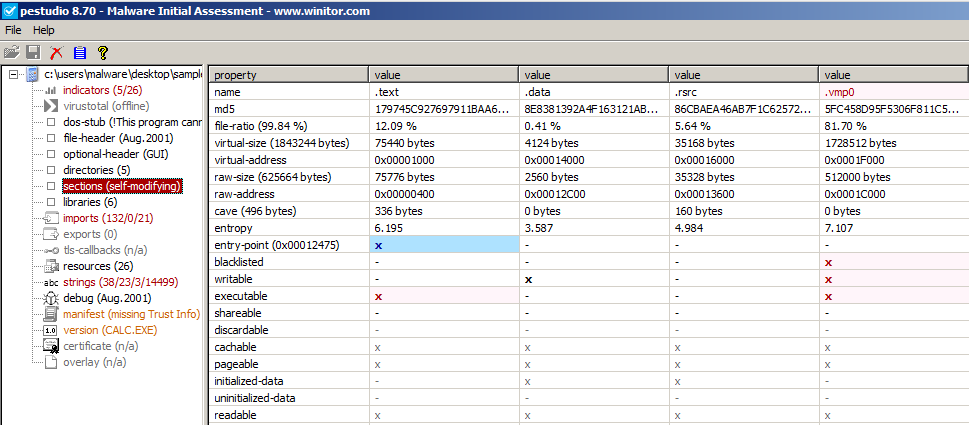
\includegraphics[width=0.5\textwidth]{img/PEStudio-sections.png}}
	\end{figure}

	The last section is the largest with a file-ratio of 81.70\%; it has an entropy greater than 7  and PEStudio marks it as blacklisted. Moreover it is both writable and executable, which is often a malicious evidence, as it indicates self modifying code.
	
	After a little search on the internet we discovered that the name ``vmp'' refers to an obfuscation program called \emph{VMProtect}\footnote{https://vmpsoft.com/}. This program cypher the code exectuting it in a virtual CPU that is different from $x86$. This code obfuscator makes the reverse engineering extremely difficult.
	
	Nevertheless, the presence of these sections allows us to suppose that the code has not been packed and its high entropy is due only to the ``vmp0'' section, which is obfuscated. In order to validate this theory, we used \emph{PEiD}, a software whose goal is to detect any possible packing. This tool provides three levels of analysis varying in depth. Every level, however, gave us the same result: ``nothing found'', meaning that PEiD could not detect any packing mechanism.

	\begin{figure}[htp]
		\frame{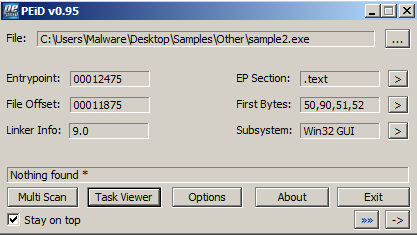
\includegraphics[width=0.5\textwidth]{img/PEiD.png}}
	\end{figure}

	\subsection{Imports}
	
	The executable imports 6 libraries in total, and in particular PEStudio marks as blacklisted 21 functions belonging to \emph{Kernel32.dll} and \emph{user32.dll}. The most interesting are:

	\begin{itemize}
		\item \textbf{getModuleHandleA}, to call external files, such as \emph{dll} or \emph{exe};
		\item \textbf{loadLibraryA}, similar to that one above;
		\item \textbf{getProcAddress}, to get the address of a procedure inside a library;
		\item \textbf{getStartupInfoA}, to get information about startup;
		\item \textbf{getCommandLineW}, to let the program execute code on the command line;
	\end{itemize}
	
	Moreover there are also imports of functions dealing with \emph{Threads}, \emph{Clipboard} and \emph{Windows}.
	This suggests a suspicious behavior, due to the possibility of the program to access to all the libraries of the installed operating system.
	In the dynamic analysis we will see what actions are actually performed.
	The figure below contains all the blacklisted imports detected by PEStudio.
	
	\begin{figure}[htp]
		\frame{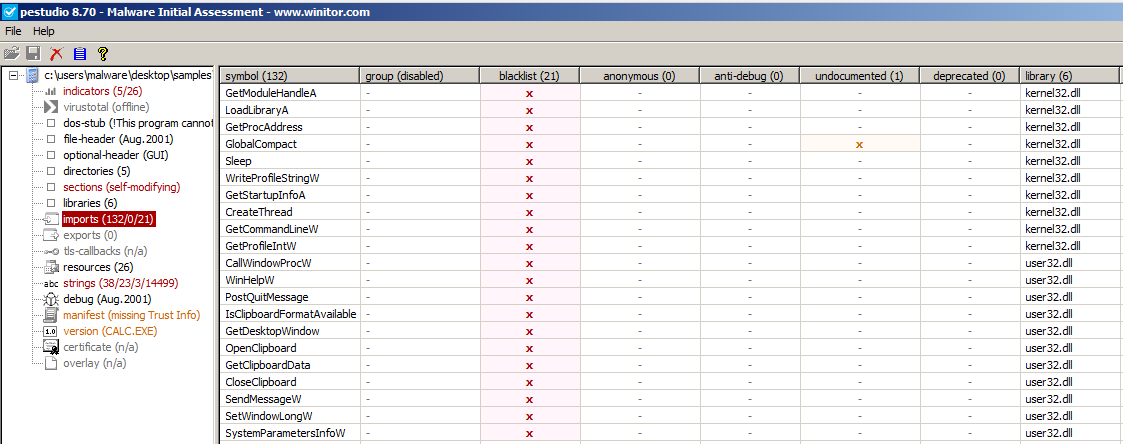
\includegraphics[width=0.5\textwidth]{img/PEStudio-imports.png}}
	\end{figure}
	
	%TODO Indicators and import analysis
	
	\subsection{Strings}
	Regarding strings we notice that those in .text, .data and .rsrc sections are in clear; furthermore many of them are function calls or values used to modify system registers.
	Followin them there are thousands of obfuscated strings, seemingly meaningless, which belong to the ``.vpm0'' section. This is another clue of code obfuscation.	
	
	
	\section{Dynamic analysis}
	
	The dynamic analysis consists of the execution of the malware in a controlled and isolated system to observe the behavior and the malicious actions performed.
	
	To accomplish this task we used \emph{VirtualBox}, a virtualization program that let us run a Windows 7 machine. VirtualBox handles the snapshots too, so that after every test the machine was restored to its initial state. The machine was also isolated from internet in order to avoid leaks.
	
	The machine was equipped with various tools to monitor the execution of the malware. The main ones were:
	\begin{itemize}
		\item \textbf{regshot}, to detect files and registers alterations between a time lapse;
		\item \textbf{procmon}, to log system functions called by the malware;
		\item \textbf{fakenet}, to track internet traffic in a simulated network.
	\end{itemize}
	These programs were executed with administrator permission in order to detect access to restricted locations.
	
	The tools can cooperate but they need to be executed is a certain schedule, in order to avoid conflicts among them. The analysis proceeded following these phases:
	\begin{enumerate}
		\item launch Fakenet;
		\item launch and setup Procmon;
		\item launch Regshot, setup path and run of its first shot;
		\item start Procmon analysis and launch of the malware;
		\item interaction with calculator by the GUI;
		\item stop Procmon tracking
		\item second Regshot shot;
		\item stop Fakenet;
	\end{enumerate}
	
	The first tests did not last too long: the GUI remained opened for just a few seconds. These tests did not give us evidence of malicious behavior, probably beacuse of the poor performance of the host machine.

	Then we ran other test leaving the malware run for a couple of minutes, leaving all the time needed to permorm bad actions. Then we collect the logs and analyzed them one by one.

	The first evidence of malicious behavior has been observed without any tools. After 20-30 seconds from the program execution the operating system prompted us a message about the \emph{Windows security center}; it was disabled and, from the control panel, it could not be re-activated. This is a seriuos threat to the security of the machine, leaving it opened to many other infections.

	\begin{figure}[htp]
		\frame{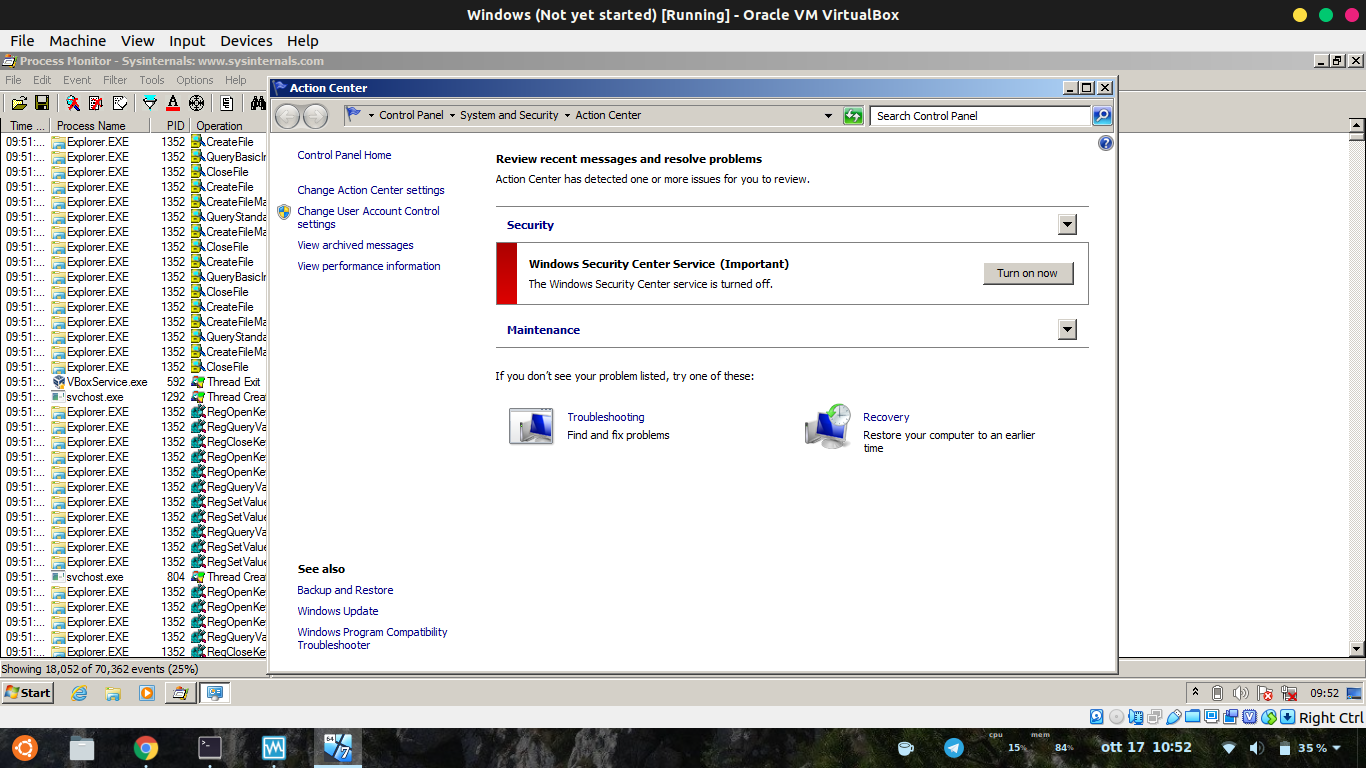
\includegraphics[width=0.5\textwidth]{img/securityCenter.png}}
	\end{figure}

	\subsection{Fakenet}

	FakeNet is a dynamic network analysis tool for malware analysts and penetration testers. It simulates a network logging the traffic generated by the machine. Every request is a file containing:

	\begin{itemize}
		\item Request type
		\item Destination URL
		\item Protocol
		\item User agent
	\end{itemize}

	The user agent field contains various informations about the local machine, such as architecture, operating system, product and so on. This string is
	\begin{quote}
		\texttt{User-Agent: Mozilla/4.0\\ (compatible; MSIE 28;\dots}
	\end{quote}
	There are other nubers dealing with the versions that have not been written for simplicity.

	The registered requests are over 900, whereas the destinations are 300, mainly russian sites. Unluckily the body is empty, and we cannot know the expected result due to the presence of Fakenet, which builds a fake http page as response to every request.

	Fakenet generated also a \emph{.pcap} file, containing the captured packets. Examinating it with \emph{Wireshark} we noticed all the TCP streams related to the POST requests, and other packets irrelevant with the malware, such as DHCP, ARP and DNS. One frequent message was a request to \emph{www.msftncs.com}, asking for a txt file called \emph{ncsi}. This sort of message is generated by Windows as a heat beat, keeping the machine constantly connected to the internet.

	This whole internet traffic should not be present, due to the absence of any socket library imported by the executable. Thus, in order to send packets over the network the malware needs to load external libraries dynamically, leaving a trace on the system that we capture using \emph{Procmon}.

	\subsection{Procmon}

	Process Monitor is an advanced monitoring tool for Windows that shows real-time file system, registry and process/thread activity. Procmon offers also a filtering function, and we set it to keep only the actions made by the malware.

	We can group these actions in 3 main sets: dll, registry and file.

	Dll stands for dynamic link library. These are files shared among all the programs of the Windows operating system which can be called to perform frequent operations. Every time that the malware loads a dll the system keeps track of the action, thus using Procmon we were able to collect them all, identifying 46 different ones called with the ``Load Image'' function. This primitive allows the program to load also other executables, but the only one loaded by the malware is the malware itself.

	Overall we measured 46 dll loaded, among wich the most interesting are the cypher family, to handle cryptography and certificates, and wbem which manages the sharing of information over the web.

	% TODO non ho ancora capito quali sono le dll che gli permettono di fare richieste POST

	Among the actions concerning with the registers Procmon logged many Open-Read-Close operations on many different ones, but only a few were written directly by the malware. These ones are about the ``Language list'' and ``Internet settings''. This last one manage the permission over the internet among the 4 different zones (Intranet, Trusted, Internet, Restricted), setting the value to 0 which means ``Accept all''. This is dangerous as exposes the machine to possible attacks over the net.
	
	Procmon registered also accesses to thousands of file, and we noticed that many one of them were infected. The infection procedure followed these steps:

	\begin{itemize}
		\item Read the \emph{.exe} victim file.
		\item Write of the content plus the infected part in a \emph{.vir} file with the same name.
		\item Copy of the content of the \emph{.vir} file to the \emph{.exe} one changing the EOF location.
		\item Set of fake information on the executable such as creation an last access time.
		\item Delete the \emph{.vir} file.
	\end{itemize}

	After the infection the victim had another section called \emph{.vmp0}, having a similar size to the original one, which is both executable and writable. The infected files are hundreds and they are stored in many different locations. Many of them are common applications such as Windows Media Player, Internet Explorer, Windows Defender, Windows Mail, Windows Photo Viewer and other files in the System32 directory.

	\subsection{RegShot}
	
	Regshot is an open-source (LGPL) registry compare utility that allows you to quickly take a snapshot of your registry and then compare it with a second one - done after doing system changes or installing a new software product.

	In our use-case we recorded the first shot just before the execution of the malware. Then we ran it for some minutes and, after the program exit, we took the second shot, saving the result of the comparison in a \emph{.txt} file.

	This file contains variuos information about registries files and folders. The downside of Regshot is that it takes care of all the system changes, but it cannot associate each change to the process that caused it, so there is no way to separate the malware generated events from the system ones. The only clue that we can use is a comparison to the logfile generated by Procmon.

	Analyzing the output there are 6 new key added to the registry, 4 related to error reporting, one to instrumentation and one to the Security Center. This last one is the most interesting because it is the trace left by the deactivation of the security center that we noticed during the malware execution. In fact among the values added to the registries there is ``Enable Notifications'' set to zero.
	Then we found all the changes reported by Procmon about the internet zones, where every value is set to 0 (Allow anything).

	Another malicious evidence that we found is that the value ``Start'' of the \emph{wscsvc} service set to 4. This service is the security center, and the value 4 stands for disabled.

	The file attributes that are modified are those related to the infected files and thus they have a different creation time.

	\section{Reverse Engineering}
\end{document}